\chapter{Requirements and Design}
\lhead{\emph{Requirements and Design}}

\section{Project Requirements}\label{project_requirements}

Functional and non-functional requirements for the solution implementation are given in the following sections \cite{Sommerville}. The requirements specification leverages terminology defined by RFC2119, \textit{Key words for use in RFCs to Indicate Requirement Levels}.

\subsection{Functional Requirements}

\begin{enumerate}
	\item \textit{(FR-1)} The software MUST support real-time rendering of message activity in a given environment.
	\item \textit{(FR-2)} The software MUST support aggregation of message activity statistics.
	\item \textit{(FR-3)} The software MUST support discovery of environment topology information.
	\item \textit{(FR-4)} The software MUST support rendering of monitored application pipeline topology structures.
	\item \textit{(FR-5)} The software MUST support parallel monitoring and discovery of multiple environments.
	\item \textit{(FR-6)} The software MUST provide an interface for user-configuration of multiple monitored environments.
	\item \textit{(FR-7)} The software MUST support a configurable retention period for monitored environment data.
\end{enumerate}

\subsection{Non-functional Requirements}
\begin{enumerate}
	\item \textit{(NFR-1)}The software MUST be extensible, supporting the addition of additional pipeline discovery and message monitoring implementations with minimal impact.
	\item \textit{(NFR-2)} The software implementation MUST be sufficiently generic to enable monitoring for environments based on disparate messaging technologies, i.e. it MUST NOT be limited to support for a single technology such as Apache Kafka.
\end{enumerate}

\section{Key Concepts and Terminology}

The following key concepts and terminology will be used for the remainder of this document.

\subsection{Environment}

An \textit{environment} is a single running instance of message-driven pipeline application comprising some number of services or microservices which communicate over a messaging system such as Apache Kafka or RabbitMQ. A \textit{monitored} environment is an environment whose topology and message activity are actively observed by the monitoring application.

\subsection{Topology}

Every environment has exactly one associated topology. A topology is either empty or represented as a directed graph, which consisting of a non-empty finite set elements called \textit{nodes} and a finite set of ordered pairs of distinct vertices called \textit{edges}\cite{GraphTheory}. A topology node corresponds to service or consumer/producer of messages in a given environment; every node has an unique associated \textit{name}. A topology edge corresponds to a message \textit{topic} in a message-driven environment; every topology edge has an associate, non-unique \textit{label}. Such a graph is depicted in Figure \ref{topology_graph}.

\begin{figure}[H]
	\centering  
	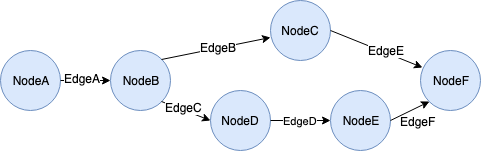
\includegraphics[scale=0.8]{figures/design/topology_graph.png}
	\caption{Example topology graph.}
	\label{topology_graph}
\end{figure}

\section{Architecture Design}

A prototype Monitoring Application will be developed. The software architecture employed will be microservices-based, as this architectural style presents certain advantages in terms of scalability, ease of development, and flexibility.

Functional requirement \textit{(FR-5)} mandates that the Monitoring Application must be capable of monitoring multiple environments simultaneously. Persistence and aggregation of monitored message activity over several environments may require significant processing and storage resources, particularly when monitoring environments containing high volumes of message activity. The horizontal scalability conferred by a microservices architecture is desirable in this case.

It is anticipated that use of a microservices architecture will afford several key advantages during development of the prototype. The inherent decoupling of responsibilities across prototype microservices will allow focused development on isolated aspects of overall application functionality. During development and testing, the ability to redeploy and debug individual services without impacting on all application functionality and availability is expected to reduce both development time and overall complexity. 

In terms of flexibility, the use of co-operating microservices communicating over HTTP enables freedom of choice in terms of language and technology choices per microservice implementation.
Five key functional areas have been identified based on the functional and non-functional requirements as presented. These are:

\begin{enumerate}
	\item Management and persistence of environment configuration and metadata.
	\item Monitoring of environment messaging activity.
	\item Aggregation of environment messaging activity.
	\item Correlation of environment messages based on some criteria.
	\item Real-time rendition of environment topology and message activity information.
\end{enumerate}

The above functional items will be implemented by the microservices enumerated in the following sections.


\subsection{Management Service}

The Management Service will be implemented as a microservice exposing a single external HTTP endpoint. The HTTP endpoint will provide a user-interface for system configuration management, in accordance with requirement \textit{FR-6}. The service will have responsibility for persistence of  application configuration, enabling user registration of monitored environment details. Per-environment discovered topology information will be also managed by this service. Data structures used to represent environment and topology state will be technology-agnostic as required by non-functional requirement \textit{NFR2}.

\subsection{Discovery Service}

The Discovery Service will be implemented as a microservice. The service will be responsible for discovery of environment topology information, in accordance with functional requirement \textit{FR-3}. The implementation will include a Discovery Agent API, which may be implemented for various topology discovery strategies. Agent implementations will be responsible for determining the topology of a given message-driven application environment. The service will be capable of discovering multiple environment topologies concurrently, in accordance with functional requirement \textit{FR-5}. To satisfy requirements \textit{NFR-1 }and \textit{NFR-2}, monitoring functionality will be pluggable, extensible and user-configurable. The Discovery Service will determine the set of monitored environments via interrogation of the Management Service.

\subsection{Monitoring Service}
The Monitoring Service, which will be implemented as a microservice, will be responsible for ingestion and persistence of messages from one or more monitored environments. Monitored message activity will be persisted on receipt, with a configurable retention period configured appropriate for real-time rendition of cluster state. The service will be capable of monitoring multiple environments concurrently, in accordance with functional requirement \textit{FR-5}. To satisfy requirements \textit{NFR-1 }and \textit{NFR-2}, monitoring functionality will be pluggable, extensible and user-configurable.

\subsection{Aggregation Service}
The Aggregation Service will be implemented as a microservice, having responsibility for real-time generation of environment summary information. Collated environment information including environment metadata and categorised message counts  per unit time will be pushed asynchronously to clients in accordance with functional requirement \textit{FR-1}. The service will be capable of aggregating data for multiple environments in parallel, in accordance with functional requirement \textit{FR-5}. The Aggregation Service will determine the set of monitored environments via interrogation of the Management Service.

\subsection{Correlation Service}
The Correlation	 Service will be implemented as a microservice, having responsibility for generation of message correlation information on monitored environments. It will expose a HTTP-based client interface.

\subsection{API Gateway}

Use of an API Gateway service is a common pattern in microservice architecture applications. It will provide a single point of access to backend services for client applications such as the Dashboard Client, masking application partitioning details.

\subsection{Client Dashboard / UI Service}

The Client Dashboard will render environment state for consumption by end-users in accordance with function requirement \textit{FR-1}. Dashboard updates - which include environment topology and environment state summary change notifications - will be pushed to the Dashboard application asynchronously.

\subsection{Service Registry}

Use of a Service Registry is a common pattern in microservice architecture applications. The registry will allow inter-service communication without the need for hard-coded host / port information.

Figure \ref{arch_high_level} depicts the overall application architecture (the UI Service and Service Registry have been omitted from this diagram).

\vspace{5mm}


\begin{figure}[H]
	\centering  
	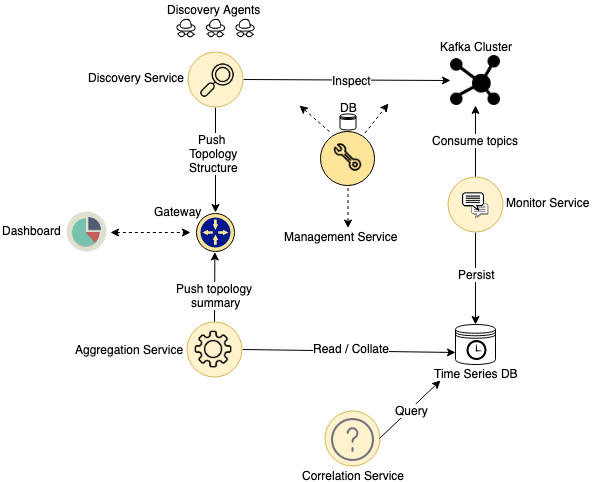
\includegraphics[width=\linewidth]{figures/design/arch_high_level.png}
	\caption{Software architecture high-level design.}
	\label{arch_high_level}
\end{figure}

\section{Design Scope}

Non-functional requirement \textit{NFR-2} mandates that the solution implementation must be sufficiently generic and extensible to support multiple messaging technologies. Plug-in interfaces will enable the implementation and addition of technology-specific discovery and monitoring implementations. For purposes of this dissertation, the author has chosen to focus on plug-in and agent implementations for a single messaging framework, namely Apache Kafka (hereafter referred to simply as Kafka)\cite{ApacheKafka}. The motivation for this choice is professional exposure to Kafka-based message processing pipelines, coupled with the contemporary ubiquity of the framework.

Kafka is an open source messaging and stream processing platform, whose key concepts include  \textit{topics}, \textit{producers} and \textit{consumers}. As the nomenclature implies, consumers and producers consume and produce Kafka messages respectively. Messages are associated with a specific, named \textit{topic}; producers and consumers may produce to and consume from multiple topics. The example topology depicted in Figure \ref{topology_graph} corresponds to a Kafka-based application as described in \ref{topology_to_kafka_mapping}.

\vspace{10 mm}

\begin{table}[H]
	\centering
	\begin{tabular}{ |p{4cm}||p{8cm}| }
		\hline
		Topology Object & Kafka Object \\
		\hline
		\textbf{NodeA}   & Producer application NodeA   \\
		\textbf{EdgeA}   & Message topic named EdgeA   \\
		\textbf{NodeB}   & Producer/consumer application NodeB   \\
		\textbf{EdgeF}   & Message topic named EdgeF   \\
		\textbf{NodeF}   & Consumer application NodeF   \\	    
		\hline
	\end{tabular}
	\caption{Topology to Kafka mapping.}
	\label{topology_to_kafka_mapping}
\end{table}

Kafka enjoys broad client language support, and as such Kafka-based environments may include applications built using Java, C/C++, Python, JavaScript, Erlang and numerous other languages. For purposes of this dissertation the author will focus on Java-based environments.

The challenges inherent to the design of functional topology discovery and monitoring plug-in implementations for a Kafka and Java based environment will be explored in the following sections.

\section{Design Challenges - Edge Correlation}

Assuming the availability of a topology model for a given environment, the following are requirements for successful monitoring and rendition of messaging activity in the environment:

\begin{enumerate}
	\item All messages generated in the monitored environment must be accessible to the monitoring application.
	\item For a given message, the monitoring application must be capable of correlating the message to a  topology edge.
\end{enumerate}

In order to successfully correlate a message to a graph edge, the monitoring application must be capable of determining the graph node responsible for production of the message. Consider the topology depicted in Figure \ref{topology_unique_edge_labels}. All edges in this topology have unique labels; thus, on observation of a Kafka message on topic \textbf{EdgeA}, it is possible to correlate that message with a single graph edge.

\begin{figure}[H]
	\centering  
	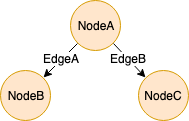
\includegraphics[scale=0.8]{figures/design/topology_unique_edges.png}
	\caption{Topology of unique edge labels.}
	\label{topology_unique_edge_labels}
\end{figure}

Now, consider the topology depicted in Figure. \ref{topology_non_unique_edge_labels}. Topolgy edge labels are non-unique; in this example, graph edges \textit{(NodeD, NodeB)} and\textit{(NodeC, NodeD)} share the edge label \textbf{EdgeC}. In order to successfully correlated a monitored message with a single topology edge, the first element of the ordered pair must be known.

\vspace{5mm}

\begin{figure}[H]
	\centering  
	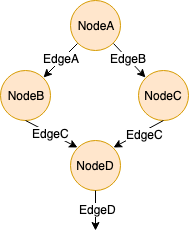
\includegraphics[scale=0.8]{figures/design/topology_non_unique_edges.png}
	\caption{Topology of non-unique edge labels.}
	\label{topology_non_unique_edge_labels}
\end{figure}

Thus, for a monitored Kafka environment in which multiple producers generate messages on a given topic, the monitoring application must determine the sender of a given message in order to successfully render message activity in the environment.

Kafka messages do not, however, identify the message sender. Figure \ref{kafka_consumer_record_api} describes the Java API for Kafka ConsumerRecord, which defines the interface to messages read by a Kafka consumer.

\begin{figure}[H]
	\centering  
	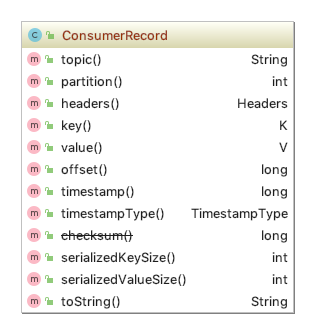
\includegraphics[scale=2.5]{figures/design/consumer_record_api.png}
	\caption{Kafka Consumer Record Java API.}
	\label{kafka_consumer_record_api}
\end{figure}

While the consumer of a message can determine the message topic, timestamp and value amongst other fields, there is no information pertaining to the producer of the message. Not only does the Kafka API not yield this information; the underlying Kafka protocol for message delivery to consumers contains no fields describing a message sender.  The protocol defines the message record structure as follows\cite{KafkaProtocol}:

\vspace{5mm}

\begin{lstlisting}[caption={Kafka Protol Message Record Definition},captionpos=b]
Record =>
Length => varint
Attributes => int8
TimestampDelta => varint
OffsetDelta => varint
KeyLen => varint
Key => data
ValueLen => varint
Value => data
Headers => [Header]

Header => HeaderKey HeaderVal
HeaderKeyLen => varint
HeaderKey => string
HeaderValueLen => varint
HeaderValue => data
\end{lstlisting}

The absence of producer information in the protocol message structure rules out approaches such as packet inspection or bytecode manipulation as a means of determining the producer of a message. 

Kafka headers have been identified as a suitable means to augment messages in order to convey producer information to message consumers. Kafka documentation describes headers as "... an API for metadata information to be added to kafka messages and a way for plugins and interceptors to add, remove, modify and otherwise act based on this metadata"\cite{KafkaHeaders}.

By augmenting all produced messages with a known header denoting the source node name, the monitoring application can successfully identify same during message consumption. Several approaches to header addition have been explored.

\subsection{Manual Header Injection} \label{manual_header_addition}

A straightforward approach to Kafka header injection involves manually updating application code to add the designated source node header to any message sent by a monitored service. The following code demonstrates the sending of a message in a Spring Boot application:

\vspace{5mm}

\begin{lstlisting}[language = Java, caption={Sending a message with Spring Kafka},captionpos=b]
public void sendMessage(final String messageData) {
Message<String> message = MessageBuilder
.withPayload(data)
.build();
template.send(message);
}
\end{lstlisting}

To add the appropriate header and value to the produced message, the code should be updated as follows, where \textit{SOURCE\_NODE\_ID} is a header name known to the monitoring environment, and \textit{APPLICATION\_NAME}, the header value, provides the unique name of the application.

\vspace{5mm}

\begin{lstlisting}[language = Java, caption={Sending a message with Spring Kafka},captionpos=b]
public void sendMessage(final String messageData) {
Message<String> message = MessageBuilder
.withPayload(data)
.setHeader(SOURCE_NODE_ID_HEADER, APPLICATION_NAME)
.build();
template.send(message);
}
\end{lstlisting}

This solution is however highly undesirable for several reasons:

\begin{enumerate}
	\item The approach is particularly invasive, requiring potentially widespread updates to producer source code. 
	\item Developers are likely to overlook the need for header addition when implementing new message producers.
	\item Ideally application source code should not have dependencies on or knowledge of any monitoring environment. 
\end{enumerate}

While this approach is undesirable, it is nonetheless an option when a less invasive means of header injection is impossible, as may be the case for Kafka producers implemented in languages such as C.

\subsection{Log Analysis}

For environments that leverage distributing tracing solutions such as Spring Cloud Sleuth, log analysis may be used to derive the sender of a given message. This approach has been evaluated in the context of Spring Boot applications. Crucially, Spring/Kafka integration code will log the production of every message before sending; the logging operation is performed by the class \texttt{org.springframework.kafka.core.KafkaTemplate}. At time of writing, the latest Spring Kafka versions will log the following information per message:

\begin{itemize}
	\item The topic name.
	\item The message key and value.
	\item The message timestamp.
\end{itemize}

Log analysis pseudocode is presented in Listing \ref{log_analysis_pseudocode}.

\begin{lstlisting}[caption={Log analysis pseudocode},captionpos=b,label={log_analysis_pseudocode}]
def getProducer(message):
for entry in log_entries:
if(entry.topic == message.topic &&
entry.timestamp == message.timestamp &&
entry.key == message.key &&
entry.value == message.value):
return entry.application_name
return NULL
\end{lstlisting}

While this approach is far less invasive than that described in Section \ref{manual_header_addition}, requiring no modifications to application source code, it does require a number of conditions to be true:

\begin{itemize}
	\item Appropriate logging levels must be set for all monitored applications.
	\item Distributed logging must be enabled.
	\item Logging configuration must include logging of the application name.
	\item Collated logs must be made available to the monitoring application (via a solution such as Logstash(Kibana).
\end{itemize}

This approach suffers from a number of limitations which impact on its feasibility; Spring Boot's logging behaviour is not guaranteed in any way and may change between releases, thus rendering log information useless. The time required to perform log analysis - as a function of log collection and scanning time - may have an adverse affect as regards real-time rendition of environment state as mandated by functional requirement \textit{(FR-1)}. Furthermore, this approach may not be applicable at all with alternate implementations such as Kafka for Python, Kafka for Node.js and others.

Finally and critically; if multiple producers dispatch identical messages to a given topic at the same instant in time - however unlikely this is - log analysis will be unable to collate the messages to a topology graph edge. 

\subsection{Header Injection via Application Framework Hooks} \label{kafka_producer_header_design}

Application frameworks may provide hooks and extension points which can be leveraged from the perspective of modifying application behaviour in a transparent and non-invasive fashion. The Spring framework provides one such hook in the form of the \textit{BeanPostProcessor}. This interface "\textit{...allows for custom modification of new bean instances, e.g. checking for marker interfaces or wrapping them with proxies.}"\cite{BeanPostProcessor}. Figure \ref{spring_bean_lifecycle} describes the various phases involved in initialisation of a Spring bean.

\vspace{5mm}

\begin{figure}[H]
	\centering  
	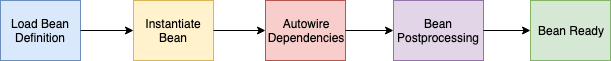
\includegraphics[scale=0.6]{figures/design/beanpostprocessor.png}
	\caption{Spring bean initialisation.}
	\label{spring_bean_lifecycle}
\end{figure}

The bean post-processing phase of bean initialisation affords an opportunity to perform customisation on Spring beans, including those involved in dispatching of Kafka message in Spring applications. One such bean type is the Spring framwork class \texttt{org.springframework.integration.channel.AbstractMessageChannel}. This abstract bean type provides methods for configuration of \texttt{ChannelInterceptor}s, documented as ".\textit{..(an) interface for interceptors that are able to view and/or modify the Messages being sent-to and/or received-from a MessageChannel}"\cite{ChannelInterceptor}.

By leveraging Spring Auto-Configuration\cite{SpringFactories} in combination with a custom bean post-processor, message headers denoting the message producer name can be transparently injected into all messages produced by a given application. Enabling this behaviour is as simple as adding an application runtime dependency to the injection library. This strategy has several advantages:

\begin{itemize}
	\item The method is minimally invasive - no modifications to source code are required.
	\item Developers of new producers are not concerned with addition of custom headers.
	\item Message consumers such as the environment monitor application can determine the sender of message with guaranteed accuracy, minimal processing time, and minimal dependencies.
\end{itemize}

This approach, if successful, will be the preferred implementation for edge correlation functionality detailed in Section \ref{software_impl_producer_ident}.

\section{Design Challenges - Topology Discovery} \label{design_topology_discovery}

\subsection{Manual Topography Configuration} \label{}

If an environment cannot be automatically discovered or only partially discovered by automated discovery agents, users of the monitoring application will require functionality enabling manual topography configuration. To this end, the Management Service will provide a client interface which enables viewing and management of environment topographies.

The topology graph depicted in Figure \ref{topology_non_unique_edge_labels} might be described by the  proposed JSON structure given in Listing \ref{topology_JSON}. A corresponding topology definition format will be defined; this format will be consumed and produced at the Management service client interface.

\vspace{5mm}

\begin{lstlisting}[caption={Sample JSON topology structure.},captionpos=b,label={topology_JSON}]
{
"nodes":[ 
{
"name": "NodeA"
},
{
"name": "NodeB"
},
{
"name": "NodeC"
},
{
"name": "NodeD"
}
],
"edges": [
{
"label": "EdgeA",
"source": "NodeA",
"target": "NodeB"
},
{
"label": "EdgeB",
"source": "NodeA",
"target": "NodeC"
},
{
"label": "EdgeC",
"source": "NodeB",
"target": "NodeD"
},
{
"label": "EdgeC",
"source": "NodeC",
"target": "NodeD"
}           
]
}
\end{lstlisting}


\subsection{Kubernetes Discovery Agent}\label{design_kubernetes_discovery_agent}

Environment topology structure may be determined from metadata extant in application deployment environments such as Kubernetes. A \textit{Kubernetes Discovery Agent} will be implemented in order to explore and demonstrate this approach.  Kubernetes (https://kubernetes.io/) is a popular open-source container orchestration system, used for management of automated application deployment and scaling. Kubernetes supports an application configuration mechanism called a \textit{ConfigMap}, a means of externalising and decoupling application configuration from application implementation and packaging, in a manner that allows the configured application to remain agnostic of the fact that it is executing in a manager Kubernetes environment.

An example Kubernetes ConfigMap is presented in Listing \ref{k8s_configmap_sample}. 

\begin{lstlisting}[caption={Kubernetes ConfigMap sample},captionpos=b,label={k8s_configmap_sample}]

kind: ConfigMap
apiVersion: v1

metadata:
name: myMicroservice-example-config
namespace: myPipeline

data:
property.key.a: propertyValue
property.key.b: propertyValue

\end{lstlisting}

Additional properties can be added to ConfigMaps at any time - including application runtime - without impacting on running applications. By adding known properties to a ConfigMap such as the example given in Listing \ref{k8s_configmap_sample}, metadata describing a subset of an application's topology graph artefacts can be made available for interrogation by third parties such as a Discovery Agent. Listing \ref{k8s_configmap_topolofy_metadata_sample} details an example of such metadata. The listed metadata describes \textbf{NodeB} and adjacent edges as given in the topology sample rendered in Figure \ref{topology_non_unique_edge_labels}.  In this proposed scheme, a topology node name is denoted by property \texttt{mon.agent.nodename} while incoming and outgoing edges are described by properties \texttt{mon.agent.incoming-edges }and \texttt{mon.agent.outgoing-edges} respectively.

\vspace{5mm}

\begin{lstlisting}[caption={Kubernetes ConfigMap containing topology metadata},captionpos=b,label={k8s_configmap_topolofy_metadata_sample}]

kind: ConfigMap
apiVersion: v1

metadata:
name: myMicroservice-example-config
namespace: myPipeline

data:
mon.agent.nodename: NodeB
mon.agent.incoming-edges: EdgeA
mon.agent.outoing-edges: EdgeC

property.key.a: propertyValue
property.key.b: propertyValue

\end{lstlisting}

The Kubernetes/Kafka Discovery Agent will be configured with the details of the Kubernetes cluster in which a given monitored application is running. Thereafter it will iteratively discover topology information using the algorithm presented by the pseudocode in Listing \ref{k8s_kafka_agent_pseudeocode}.

\vspace{5mm}

\begin{lstlisting}[caption={Kubernetes/Kafka Discovery Agent Algorithm},captionpos=b,label={k8s_kafka_agent_pseudeocode}]

for environment in monitoredEnvironments:

let topology = new Topology()

for configMap in kubernetes_namespace:
if isDiscoverable(configMap):
let nodeName = configMap.nodeName
let incomingEdges = []
let outgoingEdges = []
for topicName in configMap.consumed_topic_list:
incomingEdges.append(topicName)
for topicName in configMap.consumed_topic_list:
outgoingEdges.append(topicName)

topology.addNode(nodeName):
for(edge in incomingEdges)
topology.addEdge(edge)
for(edge in outgoingEdges):
topology.addEdge(edge)	

environment.merge(topology)
\end{lstlisting}

This approach to dynamic discovery of application topologies in Kubernetes environments  is not bound to any specific messaging technology or language implementation.

\subsection{Message Correlation Agent}\label{design_message_correlation}

In the absence of topology metadata, topology structure can nonetheless be deduced for a subset of topology structures. By correlation of related messages observed in a monitored environment a set $\theta$ of related messages may be observed. By placing a temporal ordering upon messages in the set $\theta$, it is possible to deduce the set of nodes and ordered edges that comprise a given topology. 

When related environment messages contain shared Universally Unique Identifiers (UUIDs), the set  $\theta$ is constructed trivially, by identification of observed messages with a common UUID value. While more challenging approaches to message correlation may be necessary depending on payload structures present in monitored environments, the aforementioned approach of simple field-matching correlation will be employed in the development of the monitoring application prototype.

To this end, the Correlation Service will support the implementation of a correlation-based Discovery Agent. This Agent will periodically request correlation traces from the Correlation Service; returned trace information will then be used to determine partial topology structure. 

The Correlation Service will perform correlation by determining the set of unique monitored values for a given payload field in a given environment during a moving temporal window. For each unique field value found, the service will determine the set of matching messages, ordering these by message timestamp. The service will return such traces to clients via a client interface, returning a JSON structure such as the following:

\begin{lstlisting}[caption={Correlation Service Message Trace}]
{
"messages": [
{
"edgeLabel": "edgeB",
"sourceNode": "nodeA",
"timestamp": {
"time": 1557419028600
}
},
{
"edgeLabel": "edgeC",
"sourceNode": "nodeB",
"timestamp": {
"time": 1557419028597
}
},    
{
"edgeLabel": "EdgeD",
"sourceNode": "nodeD",
"timestamp": {
"time": 1557419028602
}
}
]
}

\end{lstlisting}

Certain topology structures / monitored environments cannot be accurately discovered using this approach. Such topologies include:

\begin{itemize}
	\item Topologies in a which a single message received on a given node results in multiple messages traversing fan-out edges of the same node. In such topologies, a temporally ordered set of messages does not yield the order in which nodes are traversed.
	\item Topologies in which sink nodes do not contain fan-out edges. As messages are never observed as originating from such nodes, correlation traces processed by the correlation Discovery Agent will not contain messages indicating the existence of such a node. Similarly, any edge on which a message is never produced cannot be discovered using this approach; entire subgraphs will remain undiscovered in this circumstance.
	\item Environments in which message production time (as opposed to monitoring/consumption time) cannot be determined.  
	
\end{itemize}


\subsection{Static Code Analysis}

Static code analysis tools may be used to determine the topology of a given environment given the availability of source code for the various microservices comprising same. Common software implementation patterns may be exploited in order to determine the set of incoming and outgoing edges for a given topology node. 

In the case of Java-based Spring Boot application, consumer and producer message streams are typically configured using custom \textit{channel annotations}, which declare the existence of uniquely named message streams. An example is given in the following Java code snippet.

\vspace{5mm}

\begin{lstlisting}[caption={Spring Boot Cloud Channel Annotations}]
@Input("my.input.channel")
SubscribableChannel inboundMessages();   

@Output("my.output.channel")
MessageChannel validatedMessages();
\end{lstlisting}

Input and output channels are further configured for specific message technology using \textit{stream bindings}. For a Spring Boot microservice leveraging Apache Kafka, the input and output streams given in the previous code example might be bound as demonstrated by the following YAML snippet:

\vspace{5mm}

\begin{lstlisting}[caption={Spring Boot Cloud Channel Binding Configuration}]
spring:
cloud:
stream:
kafka:
bindings:
my.input.channel:
destination: source
contentType: application/json
my.output.channel:
destination: validated
contentType: application/json
\end{lstlisting}

Such code and configuration may be statically analysed in order to extract the set of input and output channels defined by a Spring application; by parsing the sources to all pipeline microservices, a topology structure can be derived. While this approach will not be explored any further during the development of the monitoring application, the following skeletal prototype demonstrates that static discovery of input and output channels for a Spring Boot application is not a complex task. The following code leverages the open source \textit{JavaParser} library available at https://github.com/javaparser/javaparser. Complete sources are bundled with monitoring application at \newline https://github.com/schmigware/monitoring-app.

\vspace{5mm}

\begin{lstlisting}[caption={Discovery of Spring Cloud message channels by static analysis}]
package org.cit.mcaleerj.thesis.analysis.sample;

import com.github.javaparser.JavaParser;
import com.github.javaparser.ast.body.MethodDeclaration;
import com.github.javaparser.ast.expr.AnnotationExpr;
import com.github.javaparser.ast.visitor.VoidVisitorAdapter;

import java.io.File;
import java.io.IOException;

import java.util.Optional;

public class FindStreamAnnotationSample {

public static void findStreamAnnotations(final File projectDir) {
final ProjectExplorer exp = new ProjectExplorer(new AnnotationProcessor());
exp.process(projectDir);
}

private static class AnnotationProcessor implements ProjectExplorer.FileProcessor {

public void process(final File file) {

try {
new VoidVisitorAdapter<Object>() {
@Override
public void visit(final MethodDeclaration decl, final Object arg) {
super.visit(decl, arg);
Optional<AnnotationExpr> optional = decl.getAnnotationByClass(
org.springframework.cloud.stream.annotation.Input.class);
optional.ifPresent(annotation -> {
processStreamInputAnnotation(annotation);
});
optional = decl.getAnnotationByClass(
org.springframework.cloud.stream.annotation.Output.class);
optional.ifPresent(annotation -> {
processStreamOutputAnnotation(annotation);
});
}
}.visit(JavaParser.parse(file), null);

} catch (IOException e) {
new RuntimeException(e);
}
}

private void processStreamInputAnnotation(final AnnotationExpr exp) {
//process input annotation
}

private void processStreamOutputAnnotation(final AnnotationExpr exp) {
//process input annotation
}

}

}

\end{lstlisting}

\section{Design Challenges - Topology Visualisation}\label{design_topology_visualisation}

In order to satisfy requirements \textit{FR-1} and \textit{FR-4}, the topology visualisation implementation should provide the following:

\begin{enumerate}
	\item Rendition of the most up-to-date topology structure for a monitored environment.
	\item Rendition of real-time message activity information for topology edges.
	\item Rendition of supplementary information such as environment name and edge activity snapshot time.
\end{enumerate}

A browser-based \textit{Client Dashboard} will be implemented to satisfy the above requirements. The Dashboard will render a information pertaining to a single monitored environment, using the layout proposed in Figure \ref{dashboard_high_level}. Environment name and snapshot time will convey the to users information about which environment is currently rendered, and the time at which message activity was observed. The topology itself - which is modelled internally as a digraph by the monitoring application - will likewise be rendered as a directed graph at the dashboard.

\begin{figure}[H]
	\centering  
	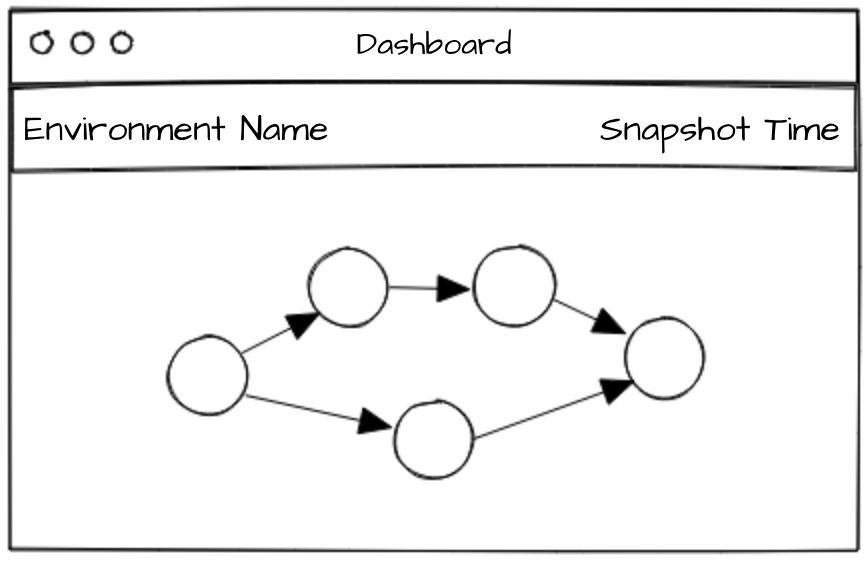
\includegraphics[scale=0.8]{figures/design/viz_high_level.png}
	\caption{High Level Client Dashboard Layout}
	\label{dashboard_high_level}
\end{figure}

\subsection{Graph Node Visualisation}\label{design_client_dashboard}

The topology graph will comprise three classes of node. Each node will be rendered using a visually distinct style.

\begin{enumerate}
	\item \textit{Topology nodes}. Such nodes correspond to discovered services (message consumers/producers) in a monitored environment. Topology nodes will be rendered using a simple, uniform and coloured geometric shape which includes the discovered node name. A proposed rendering style is demonstrated in Figure \ref{dashboard_node_high_level}.
	
	\begin{figure}[H]
		\centering  
		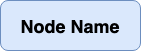
\includegraphics[scale=0.8]{figures/design/dashboard_node_high_level.png}
		\caption{Proposed Topology Node visualisation.}
		\label{dashboard_node_high_level}
	\end{figure}
	
	
	\item \textit{Source nodes}. A Source Node is added to the graph for every graph edge which has no discovered topology node as its discovered source node. Such an edge might represent incoming messages from an external system. No node label is rendered for such nodes, which will be rendered using an identifiable, uniquely styled geometric shape such as that proposed in Figure  \ref{dashboard_source_node_high_level}.
	
	\begin{figure}[H]
		\centering  
		
\includegraphics[scale=0.8]{figures/design/dashboard_source_node_high_level.png}
		\caption{Proposed Source Node visualisation.}
		\label{dashboard_source_node_high_level}
	\end{figure}
	
	\item \textit{Sink nodes}. A Sink Node is added to the graph for every graph edge which has no discovered topology node as its target node. Such an edge might represent messages outgoing to an external system.  No node label is rendered for such nodes, which will be rendered using an identifiable, uniquely styled geometric shape such as that proposed in Figure  \ref{dashboard_sink_node_high_level}.
	
	\begin{figure}[H]
		\centering  
		
\includegraphics{figures/design/dashboard_sink_node_high_level.png}
		\caption{Proposed Sink Node visualisation.}
		\label{dashboard_sink_node_high_level}
	\end{figure}
\end{enumerate}

\subsection{Graph Edge Visualisation}
Graph edges will be rendered using directed arrows. Each edge will be labelled with:

\begin{itemize}
	\item  The associated edge name, corresponding to for instance a message topic name in a monitored Kafka environment.
	\item An activity summary, displaying the number of messages monitored per second on the given edge. 
\end{itemize}

The proposed rendition for a topology edge is depicted in Figure \ref{dashboard_edge_high_level}.
\vspace{5mm}

\begin{figure}[H]
	\centering  
	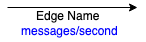
\includegraphics{figures/design/dashboard_edge_high_level.png}
	\caption{Proposed Edge visualisation.}
	\label{dashboard_edge_high_level}
\end{figure}

\subsection{Rendering Real-Time Topology Structure and Activity}

Monitored environment topology discovery and activity aggregation will be performed on an ongoing and real-time basis by various backend services. The Client Dashboard will subscribe to these services for asynchronous notifications pertaining to topology structure changes and edge activity information. Such information will be rendered on receipt by the client. 

\section{Software Development Methodology}\label{design_methodology}

The Waterfall model\cite{Palmquist13parallelworlds} will be employed during development of the monitoring prototype. Given the solution will be implemented as a set of microservices, the methodology will be applied in an iterative fashion. Initially, the contracts between co-operating microservices will be identified. Thereafter, the Waterfall model will be applied to the implementation of each service in turn. The order in which the various components will be implemented is expected to flow as follows, respecting the dependencies between services.

\begin{enumerate}
	\item Service Registry 
	\item Management Service
	\item Monitoring Service
	\item Monitoring task implementation(s)
	\item Aggregation Service
	\item Correlation Service
	\item Discovery Service
	\item Discovery Agent implementation(s)
	\item Gateway Service
	\item UI Service / Dashboard Client
\end{enumerate}

It is anticipated that some retrospective design and implementation revision will be necessarily undertaken during development of the solution.

Successful implementation of the solution will depend on application of an existing software development skill-set and knowledge base, which will be augmented by developing a working knowledge of several technologies including:

\begin{itemize}
	\item Spring Boot 2.0
	\item D3 Visualisation Framework  
	\item WebSocket API
	\item GraphQL API
	\item Kubernetes / Minikube
\end{itemize}

\section{Software Evaluation}\label{design_evaluation}

The success of the software prototype will be evaluated in term of the use case set out in the opening chapter of this thesis: 

\textit {As a developer, I want to understand the composition and activity state of my deployed pipeline applications at a glance}.


